\documentclass[11pt]{article}
\usepackage{coling2018}
\usepackage{times}
\usepackage{url}
\usepackage{latexsym}
\usepackage[utf8]{inputenc}
\usepackage{graphicx}
\usepackage{xcolor}

\title{Deconvolution for linguistic analysis}

\author{
L. Vanni\textsuperscript{1}, M. Ducoffe\textsuperscript{2}, D. Mayaffre\textsuperscript{1}, F. Precioso\textsuperscript{2}, D. Longrée\textsuperscript{3}, V. Elango\textsuperscript{2}, N. Santos \textsuperscript{2}, J. Gonzalez \textsuperscript{2}, L. Galdo \textsuperscript{2}\\
  \textsuperscript{1} Univ. Nice Sophia Antipolis - I3S, UMR UNS-CNRS 7271 06900 Sophia Antipolis, France \\
  \{lvanni, mayaffre\}@unice.fr \\
  \textsuperscript{2} Univ. Nice Sophia Antipolis - BCL, UMR UNS-CNRS 7320 - 06357 Nice CEDEX 4, France \\
  \{ducoffe, precioso\}@unice.fr - ecveer@gmail.com \\
  \textsuperscript{3} Univ. Liège - L.A.S.L.A, Bélgique \\
  dominique.longree@uliege.be\\}
\date{}

\begin{document}
\maketitle



\begin{abstract}
  This document contains the instructions for preparing a paper submitted
  to COLING-2018 or accepted for publication in its proceedings. The document itself
  conforms to its own specifications, and is therefore an example of
  what your manuscript should look like. These instructions should be
  used for both papers submitted for review and for final versions of
  accepted papers. Authors are asked to conform to all the directions
  reported in this document.
\end{abstract}

\section{Introduction}
As many other fields of data analysis, Natural Language Processing (NLP) has been strongly impacted by the recent advances in Machine Learning, more particularly with the emergence of Deep Learning techniques. These techniques outperform all other state-of-the-art approaches on a wide range of NLP tasks and so they have been quickly and intensively used in industrial systems. Such systems rely on end-to-end training on large amounts of data, making no prior about the linguistic structure and focusing on stastically frequent patterns. Thus, they somehow step away from computational linguistics as they learn implicit linguistic information automatically without aiming at explaining or even exhibiting classic linguistic structures underlying to the decision.

This is the question we raise in this article and that we intend to address by exhibiting classic linguistic patterns which are indeed exploited implictly in deep architectures to lead to higher performances.
Do neural networks make use of co-occurrences and other standard features, considered in traditional Textual Data Analysis (TDA)? 
Do they also rely on complementary linguistic structure, unreachable by the traditional techniques? If so, projecting neural networks 
features back onto the input space would highlight new linguistic structures would lead to improving the analysis of a corpus and a better understanding on where the power of the deep learning techniques comes from.
Our hypothesis is that deep learning is, of course, sensitive to the linguistic units on which the computation of the key statistical sentences are based, but also sensitive to other phenomena than frequency and other complex linguistic 
observables that the TDA has more difficult to take into account - as would be linguistic patterns (Mellet et Longrée, 2009).
Our contribution confronts Textual Data Analysis and Convolutional Neural Networks for text analysis. 
We hijack deconvolution network for image analysis to offer to the linguistic community a new point of view for text analysis that we denote deconvolution saliency. Our deconvolution saliency corresponds to the sum over the 
word embedding of the deconvolution projection of a given feature map. Such score provides a heat-map over 
words in a sentence that promotes the patterns impacting for the classification decision.
We confront z-scoring and deconvolution saliency on three languages: English, 
French and Latin. For all our datasets, deconvolution saliency highlights new linguistic observables, unperceivable with z-scoring.




\section{Related work}

Convolutional Neural Networks (CNNs) are widely used in the computer vision community for a wide panel of tasks: ranging from image classification, 
object detection to semantic segmentation. It is a bottom-up approach where we apply on an input image, stacked layers of convolutions, non-linearities and sub-sampling.
Encouraged by the success for vision tasks, researchers applied CNNs to text-related problems. The use of CNNs for sentence modeling traces back to (Col-
lobert and Weston, 2008). Collobert adapted 
CNNs for various NLP problems including Part-of-Speech tagging, chunking, Named Entity Recognition and semantic labeling (cite). 
CNNs for NLP work as an analogy between an image and a text representation. Indeed each word is embedded in a vector representation, then several words build a matrix (concatenation of the vectors). 

% \textcolor{red}{Fred: La ligne qui suit est trop detaillee pour etre la et on ne voit pas le lien avec le reste du paragraphe}
% \textcolor{green}{Melanie: on peut l'utiliser dans la description du modele}
% Word embeddings are not intended to hold spatial information. Thus the width of the convolutional filters is usually the same as the dimension of the word features.

We first discuss our choice of architectures. 
If Recurrent Neural Networks (\textit{mostly GRU and LSTM}) are known to perform well on a broad range of tasks for text, recent comparisons have confirmed the advantage of CNNs 
over RNNs when the task at hand is essentially a keyphrase recognition task [1]. Recognition task is at the heart of linguistic interests which mostly focus on contrastive analysis.
Moreover, CNNs are static architectures that, according to specific tuning, are more robust 
to vanishing gradient and thus can also model long-term dependency in a sentence (Dauphin et al.,  
Wen et al. (2016) and Adel and Schutze (2017)). 
% \textcolor{red}{Fred: Encore, la ligne qui suit est trop detaillee pour etre la et on ne voit pas le lien avec le reste du paragraphe}
% Due to the convolution operators involved, 
% they can be easily parallelized and may be also inferred on CPU, which is a practical solution to get rid of the need of GPUs at test time and widespread our tools.

 All previous works converged to a common assessment: both CNNs and RNNs provide relevant, but different information for text classification. 
 However, if several works have studied linguistic structures inherent in RNNs, to our knowledge, none of them have focused on CNNs. 
 A first line of research has extensively studied the interpretability of word embeddings and their semantic representations (cite). 
 When it comes to deep architectures, Krizhevsky et al. (cite) used LSTMs on character level language as a testbed. They demonstrate the existence of 
 long-range dependencies on real word data. Their analysis is based on gate activation statistics and is thus global. On another side, Li et al. (cite)
 provided new visualization tools for recurrent models. They use decoders, t-SNE and first derivative saliency, in order to shed a light on how neural models work.
Our perspectives differ from their line of research, as we do not intend to explain how CNNs work on textual data, but rather use their features 
to provide complementary information for linguistic analysis.

Although the usage of RNNs is more common, there exist many visualization tools for CNNs analysis, 
inspired by the computer vision field. Such works may help us highlighting the linguistic features learned by a 
CNN. Consequently, our method takes inspiration from those works. Visualization models in computer vision mainly consist 
in inverting latent representations in order to spot active regions or features that are relevant to the classification decision.
One can either train a decoder network or used backpropagation on the input instance to highlight its most relevant features. 
While those methods may hold accurate information in their input recovery, they have two main drawbacks: 
i) they are computationally expensive : the first method requires to train a model for each latent representation, and the second relies 
on backpropagation for each submitted sentence. ii) they are highly hyperparameters’ dependent and may require some tuning given the task at hand.
On the other hand, Deconvolution Networks, proposed by Zeiler et al in ?, is an off the shelf method to project a feature map in the input 
space. It consists in inverting each convolutional layer iteratively, back to the input space. The inverse of a discrete convolution is 
computationally challenging. In response, a coarse approximation may be employed which consists of inverting channels and filters weights 
in a convolutional layer and then transposing their kernel matrix. More details of the deconvolution heuristic are provided in section~\ref{sec:method}.
Deconvolution holds several advantages. Firstly it induces minimal computational requirements compared to previous visualization methods. 
Also, it has been used with success for semantic segmentation on images: in ?; Noh et al demonstrate the efficiency of deconvolution networks 
to predict segmentation masks to identify pixel-wise class labels. Thus deconvolution is able to localize meaningful structure in the input space.


\section{Model}

\subsection{Text Classification}

We propose a deep neural model to capture linguistics paterns in text. This model is based on simple Convolutional Neural Network models with an embedding layer for word representaions, one convolutional with pooling layer and finaly one dense layer. Figure \ref{cnn} shows the global structure of our architecture. The input is a sequence of words $ w_{1}, w_{2} ... w_{n} $ and the output contains class elements (for text classification). The embedding is built on top of a Word2Vec architecture trained on a Skip-gram model. Our text tokenizer keeps all the words to make sure all linguistic material is detected at the end by the model. This embedding is also modifiable by the model to attain optimal text-classification acuracy. 

The Convolutional layer is based on a two-dimensional convolution, the same as used for picture convolution, but with a fixed width corresponding to the max width (this size is actually equal to the embedding size). With this setting, our usage of the two-dimensional convolution is in reallity the same as a one-dimensional convolution (the default convolutionnal layer for text). The only parameter we adjust here is the height of the filter corresponding to the number of words we want to put in the filter. The goal of this approach is to be able to use the standard picture deconvolution (conv2D Transpose) methods for our model on text.

The last layer is a fully connected dense network (with one hidden layer) finishing on a output size corresponding to the number of classes we attempt to train.

\begin{figure}[h]
\begin{center}
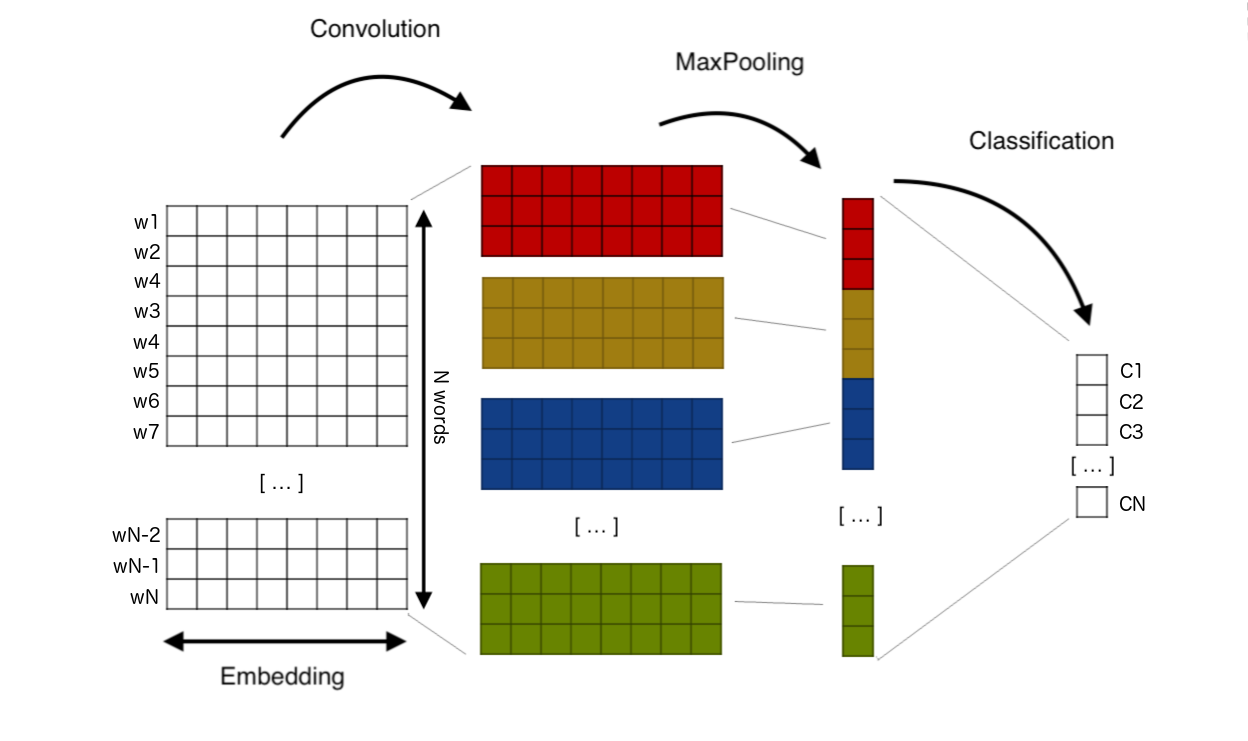
\includegraphics[width=8cm]{img/model_classif.png}
\caption{CNN model}
\label{cnn}
\end{center}
\end{figure}

\subsection{Deconvolution}

Since we use same architecture as image detection, making a deconvolutional layer is really straightforward. There are several methods to visualize the deep internal mecanisms of a neural network. One is known as convolutional transposed. Our deconvolutional network use the same embedding and convolution layer as we use for the classification but we replace the finale dense layer by a convolutional transposed layer (also called deconvolution). After we trained the model we setup the weight of each neuron of the deconvolutional network with the learned weights of the classification network. The result is a new network that takes as input a sequence of words and gives as output all the trained filters of the text classification applied on the given sequence. Then the activation score of each word is calculated as shown in Equation \ref{equation} with $x$ is the size of the embedding, and $y$ the number of applied filters : 

\begin{equation}
\mathop{\sum^{x}\sum^{y}}_{i=1  j=1}  a_{ij} = s_{n}
\label{equation}
\end{equation}

\begin{figure}[h]
\begin{center}
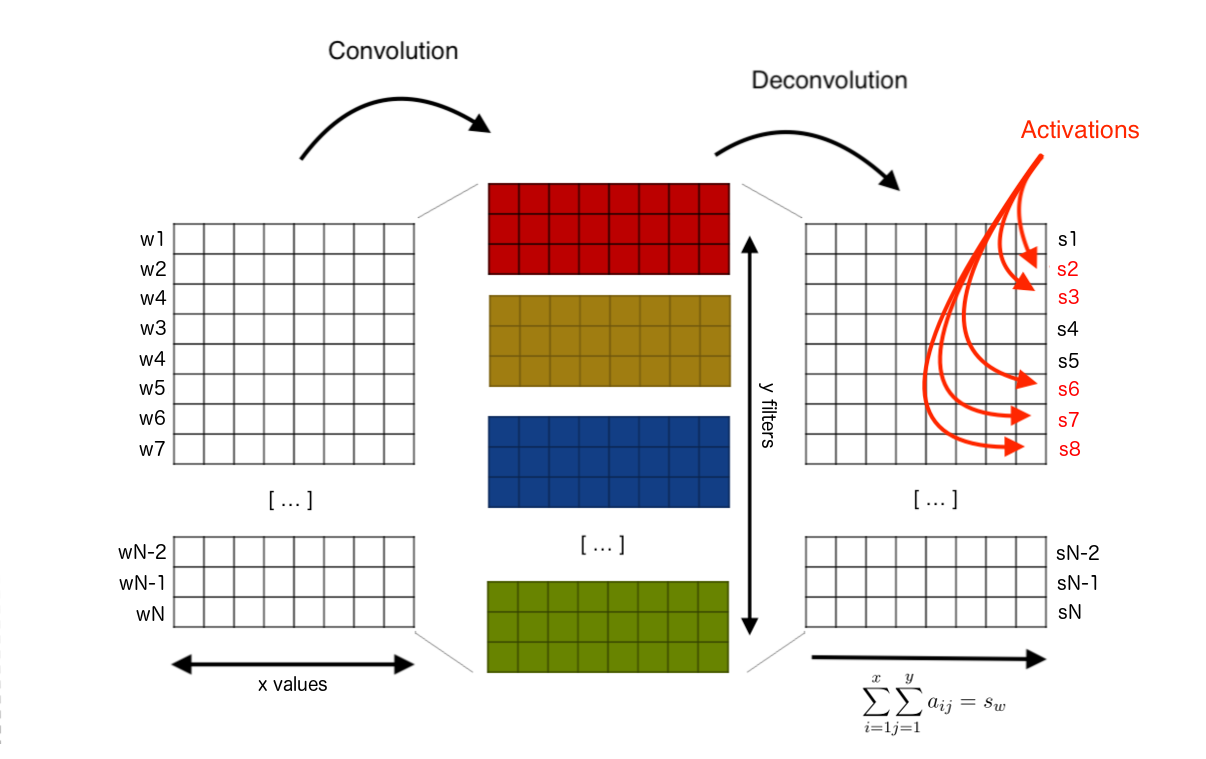
\includegraphics[width=8cm]{img/model_deconv.png}
\caption{Deconvolution model}
\label{cnn}
\end{center}
\end{figure}

With this method we are able to show a sort of topology of a sequence of words. All words have an unique activation score related to the others. We will see now that this output of the deconvolution gives us much information on how the network makes its final descision (prediction). There are well known linguistic marks encoded inside the networm, as well as more complex patterns based on co-occurrences and possibly also on grammatical and syntaxic analysis.


\section{Experiments}

\subsection{Z-score Versus Activation-score}

Z-score is one of the most used methods in linguistic statistics. It compares the observed frequency of a word with the frequency expected in case of a "normal" distribution. This calcul gives easily for example the most specific vocabulary of a given author in a contrastive corpora. The highest z-score are the most specific word in this case. This is a simple but strong method to analyze feature on text. It can be also used to classify word sequences according to the global z-score (sum of the score) in the sequence. The mean accuracy of this methods on our data set is around 85\%, that confirm z-score is really meaningful on contrastive data. On the other hand, the deep learning reaches most of time more than 90\% on text classification. It means the training methods can learn also by themselves some sort of linguistic specificities useful to distinguish class of text or authors. We've seen on image that's the role of the convolution. It learns an abstraction on the data to make classification easier. The question is : what is the nature of this abstraction on text ? We going to seen now that the deep learning detect automatically words with hight z-score but apparently it's not this only linguistic marks detected.

\begin{figure}[h]
\begin{center}
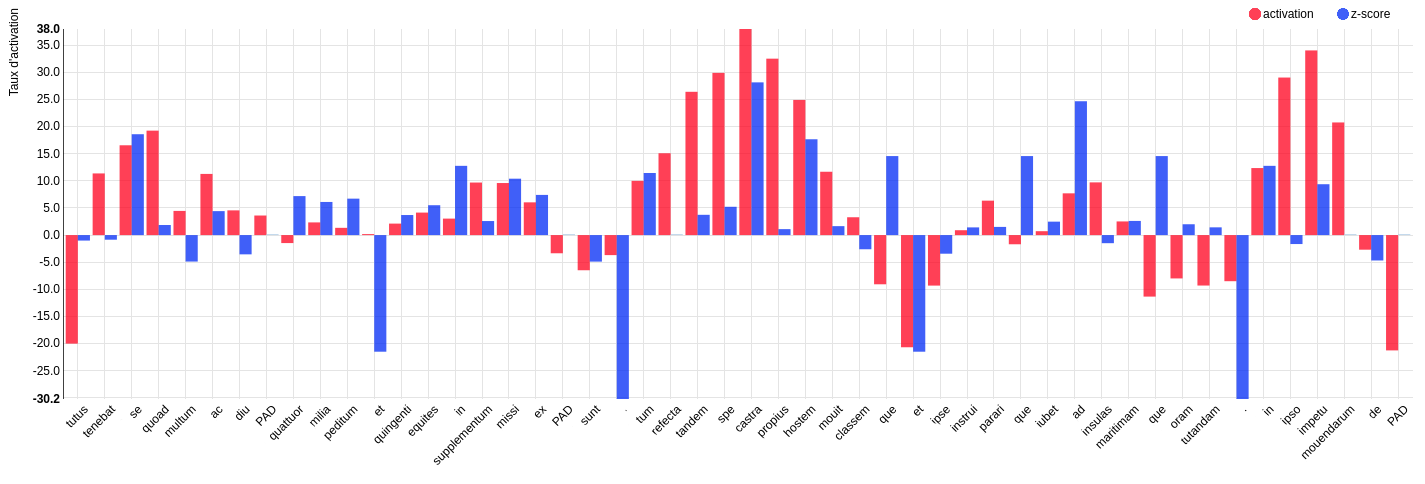
\includegraphics[width=16cm]{img/z-score_activations.png}
\caption{Latin dataset : Livius Book XXIII Chap. 26 - Z-score Vs Activation-score}
\label{comparision}
\end{center}
\end{figure}

The Figure \ref{comparision} shows us a comparison between z-score and activation-score on a sequence extract form our latin corpora. Here it's an example where Livius\footnote{Lucius Livius Andronicus (c. 284 – c. 205 BC) was a Greco-Roman dramatist and epic poet of the Old Latin period} use some specific words. As we can see, when the z-score is the highest the activation-score around is also very high (word \textit{castra}). But not always, for example small words as \textit{que}, \textit{ad} and \textit{et} are also high in z-score but they not activate the network as the same level. We saw in (reference ****) that deeplearning is more sensible with long words, but we can see also on Figure \ref{comparision} that word like \textit{tenebat}, \textit{multum} or \textit{propius} are totally uncorrelated. If we make the Pearson\footnote{Pearson correlation coefficient measures the linear relationship between two datasets. It has a value between $+1$ and $-1$, where $1$ is total positive linear correlation, $0$ is no linear correlation, and $-1$ is total negative} correlation coefficient on this sequence, we obtain 0.38. Not a hight correlation so, and this example one of the most correlated example of our dataset.

\subsection{Dataset : English}

\begin{quote}
\textit{[...] \textcolor{red}{\textbf{i enjoyed three moments}} in the film in total , \textcolor{red}{\textbf{and if i am being honest and}} the person \textcolor{red}{\textbf{next to me fell asleep}} in the middle and started PAD during the slow space chasescenes . \textcolor{red}{\textbf{the story failed to}} draw me in and entertain \textcolor{red}{\textbf{me the way}} [...]} 
\end{quote}

Pos : 

    film : 5.28
    and : 12.23 (x4)
    honest : 4
    entertain : 2.4

Neg:

    cooccurrence : 
        "and if" et honest
        "LEM:fall" et asleep
        story :  -1.61  ;   failed : 1.94    mais "NN LEM:fail" : 4.25


\subsection{Dataset : French}

\begin{quote}
\textit{[...] notre pays \textcolor{red}{\textbf{advienne à}} l'école pour nos enfants, au travail pour l' ensemble de \textcolor{red}{\textbf{nos concitoyens}} pour le climat pour le quotidien de chacune et chacun d' entre vous . \textcolor{red}{\textbf{Ces transformations profondes}} ont commencé et se \textcolor{red}{\textbf{poursuivront}} avec la même force le même rythme la même intensité [...]} 
\end{quote}

This excerpt from the speech of Emmanuel Macron (31 December 2017) is poorly attributed by the ADT (Z-score) which brings it statistically closer to De Gaulle, and well attributed by the Deep learning that recognizes Macron.
The error of statistical attribution can be explained by a Gaullist phraseology and the multiplication of linguistic markers strongly indexed by de Gaulle: for example, de Gaulle had the characteristic of making long and literary sentences articulated around conjunctions of coordination as " and "(z-score = 28 for de Gaulle, 2 occurrences in the excerpt). His speech was also more conceptual than the average, and this resulted in an over-use of the articles defined (the, the, the, the) very numerous in the extract (7 occurrences); especially in the feminine singular ("the" Republic, "the" freedom, "the" nation "," the "war, etc., here" the "same force," the "same intensity).

The best performances of deep learning question the linguist and marry perfectly what we know socio-linguistically dynamic speech of Macron.

The most important activation zone of the extract concerns the noun phrase "deep transformation".
Taken separately, none of the two words of the phrase are very Macronian from a statistical point of view ("transformation" = XXX "deep" = YYY). Better: the syntagm itself is not attested in the corpus of learning of the President (0 occurrence).
However, it can be seen that the co-occurrence of "transformation" and "deep" amounts to + XXX at Macron: so it is not the occurrence of one word alone, or the other, which is Macronian but the simultaneous appearance of both in the same window.
However, the co-occurrence of "transformation" and "profound" can not be sufficient to characterize Macron, especially because the co-occurrence of the two words is more frequent at Pompidou for example; other summed indices are required for allocation.
The second and complementary activation zones of the extract thus concern the two verbs "come" and "will continue".
From a semantic point of view, the two verbs perfectly conspire, after the phrase "profound transformation", to give the necessary dynamic to a discourse that advocates change. But it is the verb tenses (borne by the morphology of the verbs) that appear to be determining in the analysis.
The calculation of the grammatical codes co-occurring with the word "transformation" thus indicates that the verbs in the subjunctive and the verbs in the future (and also the nouns) are the privileged codes at Macron. (GRAPH XXX)
More precisely, the algorithm indicates that, in Macron, when "transformation" is associated with a verb in the subjunctive (here "come"), then there is usually a verb in the future co-present (here "will continue") .
"Transformation deep", "to come" to the subjunctive, "to continue" to the future: all these elements sign, together, a speech made of promise of action, in the mouth of a young and dynamic president.
Finally, the graph indicates that "transformation" is especially associated with names in the President: in an extraordinary concentration, the extract lists 11 ("country", "school", "children", "work", "fellow citizens"). , "climate", "daily", "transformations", "force", "rhythm", "intensity").

\subsection{Dataset : Latin}

\begin{quote}
\textit{[...] tutus tenebat se quoad multum ac diu PAD quattuor milia peditum et quingenti equites in supplementum missi ex PAD sunt . tum refecta tandem spe \textcolor{red}{\textbf{castra propius hostem}} mouit classem que et ipse instrui parari que iubet ad insulas maritimam que oram tutandam . in \textcolor{red}{\textbf{ipso impetu}} mouendarum de [...]} 
\end{quote}

As historians, Caesar and Livy share a number of specific words:
- tool words, here (reflexive pronoun) -que (= "and", a coordinator), prepositions in "in", ad "to", ex "out of"
- names like equites "the riders" or "castra" the camp

The attribution of the sentence to Caesar can not rest on the specificities - that or in or castra, with differences equivalent or inferior to Livy. On the other hand, the differences of se, ex, are superior, as that of equites. Two very Caesarian terms undoubtedly make the difference iubet ("he orders") and ("milia" thousands).

The superior deviations of quattuor ("four"), "castra", "hostem" (the enemy), "impetu" ("the assault") at Titus Live are not enough to switch the attribution to this author .

On the other hand, the Deep Learning "activates" as "liviennes" several zones appearing at the beginning of sentence and corresponding to coherent syntactic structures:

- Tandem reflexes spe castra propius hostem mouit ": then the hope having finally returned, it approaches the camp closer to the camp of the enemy".

despite the fact that castra in hostem mouit is attested only by Tacitus

- in ipso metu: in fear itself ", while in X metu is attested 1x at Caesar and once at Quinte-Curce.

The hypothesis here is twofold:

- the structure tum + participates Ablative Absolute (tum refecta) is more characteristic of Titus Live (3.3, 8 occurrences) than of Caesar (1.7: 3 occurrences), even if it is even more specific of Tacitus (4 , 2: 10 occurrences).

- co-perpetratory castra and impetu networks may also have played a role:

impetu:
- in Titus Live, appear as cooccurrents lemmas HOSTIS 9.42 and CASTRA 6.75, while HOSTIS only has a gap of 3.41 in Caesar and that CASTRA does not appear in the list of cooccurrents impetu

castra:
the first cooccurent at Titus Live is HOSTIS (22,72), before CASTRA (10,18), AD (10,85), IN (8,21), IMPETVS (7,35), -QUE (5,86) )
while in Caesar, IMPETVS does not appear and the scores of all other lemmas are lower except CASTRA (15,15): HOSTIS (8),, AD (10,35), IN (5,17), - THAT (4.79)



\section{Conclusion}

ADT and deep learning may not be foreign continents to each other \ citep {lebart1997}. This contribution by crossing statistical approach and neural network allowed us to identify key passages and perhaps reasons that could feed our textual treatments. If the observables that presided over the detection of key passages by the ADT (the lexical specificities) are known and tested, the zones of activation of the deep learning seem to raise new linguistic observables. Recall that the linguistic matter and the topology of the passages can not return to chance: the zones of activations make it possible to obtain recognition rates of more than 90 \% on the French political speech and 85 \% on the corpus of the LASLA ; either rates equivalent to or higher than the rates obtained by the statistical calculation of the key passages. It remains to improve the model and to understand all the mathematical and linguistic outcomes. The first improvement that we now propose to implement is the injection of morphosyntactic information into the network in order to test ever more complex linguistic patterns.


%\bibliographystyle{acl}
%\bibliography{biblio}
% \begin{thebibliography}{}
% 
% \bibitem[\protect\citename{Aho and Ullman}1972]{Aho:72}
% Alfred~V. Aho and Jeffrey~D. Ullman.
% \newblock 1972.
% \newblock {\em The Theory of Parsing, Translation and Compiling}, volume~1.
% \newblock Prentice-{Hall}, Englewood Cliffs, NJ.
% 
% \bibitem[\protect\citename{{American Psychological Association}}1983]{APA:83}
% {American Psychological Association}.
% \newblock 1983.
% \newblock {\em Publications Manual}.
% \newblock American Psychological Association, Washington, DC.
% 
% \bibitem[\protect\citename{{Association for Computing Machinery}}1983]{ACM:83}
% {Association for Computing Machinery}.
% \newblock 1983.
% \newblock {\em Computing Reviews}, 24(11):503--512.
% 
% \bibitem[\protect\citename{Chandra \bgroup et al.\egroup }1981]{Chandra:81}
% Ashok~K. Chandra, Dexter~C. Kozen, and Larry~J. Stockmeyer.
% \newblock 1981.
% \newblock Alternation.
% \newblock {\em Journal of the Association for Computing Machinery},
%   28(1):114--133.
% 
% \bibitem[\protect\citename{Gusfield}1997]{Gusfield:97}
% Dan Gusfield.
% \newblock 1997.
% \newblock {\em Algorithms on Strings, Trees and Sequences}.
% \newblock Cambridge University Press, Cambridge, UK.
% 
% \end{thebibliography}

\end{document}
